\RequirePackage{luatex85}
\documentclass[tikz,border=0]{standalone}
\usepackage[no-math]{fontspec}
\setmainfont[Ligatures=TeX]{PragmataPro-Bold}
\usetikzlibrary{bayesnet,positioning,backgrounds,fit,shapes.geometric,calc}
\definecolor{bgColor}{RGB}{38,50,56}
\definecolor{textColor}{RGB}{195,206,227}
\definecolor{nodeColor}{RGB}{195,206,227}
\definecolor{edgeColor}{RGB}{195,206,227}
\begin{document}
  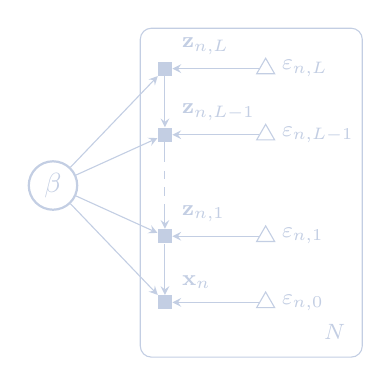
\begin{tikzpicture}[textColor]
  	\tikzstyle{latent} = [circle,draw=nodeColor,thick,inner sep=2pt,minimum size=1.75em,node distance=1]
  	\tikzstyle{obs} = [latent,draw=nodeColor,fill=textColor,fill opacity=.25,text opacity=1]
  	\tikzstyle{factor} = [rectangle,fill=nodeColor,minimum size=.5em,inner sep=0pt,node distance=0.4]
    \tikzstyle{noise} = [regular polygon,regular polygon sides=3,draw=nodeColor,fill=none,minimum size=.75em,inner sep=0pt,node distance=0.4]
    \tikzstyle{plate} = [draw,rectangle,rounded corners,inner sep=6pt,fit=#1]
  	\tikzset{>={stealth}}

    \factor [factor] {xn} {30:$\mathbf{x}_n$} {} {};
    \factor [noise, right=1.1cm of xn] {epsn} {right:$\mathbf{\varepsilon}_{n,0}$} {} {};
    \edge {epsn} {xn};

    \factor [factor, above=.65cm of xn] {zn1} {30:$\mathbf{z}_{n,1}$} {} {};
    \edge {zn1} {xn};
    \factor [noise, right=1.1cm of zn1] {epsn1} {right:$\mathbf{\varepsilon}_{n,1}$} {} {};
    \edge {epsn1} {zn1};

    \coordinate[above=.225cm of zn1] (zn2);
    \edge {zn2} {zn1};

    \coordinate[above=.725cm of zn2] (znLm2);
    \edge [-,dashed] {znLm2} {zn2};

    \factor [factor, above=.15cm of znLm2] {znLm1} {30:$\mathbf{z}_{n,L-1}$} {} {};
    \edge [-] {znLm1} {znLm2};
    \factor [noise, right=1.1cm of znLm1] {epsnLm1} {right:$\mathbf{\varepsilon}_{n,L-1}$} {} {};
    \edge {epsnLm1} {znLm1};

    \factor [factor, above=.65cm of znLm1] {znL} {30:$\mathbf{z}_{n,L}$} {} {};
    \edge {znL} {znLm1};
    \factor [noise, right=1.1cm of znL] {epsnL} {right:$\mathbf{\varepsilon}_{n,L}$} {} {};
    \edge {epsnL} {znL};

    \node [latent, left=1.1cm of $0.5*(xn) + 0.5*(znL)$] (beta) {$\mathbf{\beta}$};
    \edge {beta} {xn,zn1,znLm1,znL};

    \coordinate[right=.925cm of epsn] (rightofepsn);
    \coordinate[above=.2cm of znL] (aboveofznL);
    \plate {epsnxn} {(xn)(aboveofznL)(epsnL)(rightofepsn)} {$N$};

  \end{tikzpicture}
\end{document}